% Created 2015-09-08 Tue 12:27
\documentclass[11pt]{article}
\usepackage[utf8]{inputenc}
\usepackage[T1]{fontenc}
\usepackage{fixltx2e}
\usepackage{graphicx}
\usepackage{longtable}
\usepackage{float}
\usepackage{wrapfig}
\usepackage{rotating}
\usepackage[normalem]{ulem}
\usepackage{amsmath}
\usepackage{textcomp}
\usepackage{marvosym}
\usepackage{wasysym}
\usepackage{amssymb}
\usepackage{hyperref}
\tolerance=1000
\author{Giulio Bottazzi}
\date{\today}
\title{gbutils: command line econometrics}
\hypersetup{
  pdfkeywords={},
  pdfsubject={pippa lippa},
  pdfcreator={Emacs 24.3.1 (Org mode 8.2.4)}}
\begin{document}

\maketitle
\tableofcontents



\section{Getting Started}
\label{sec-1}

This is a brief description of \texttt{gbutils} (version 5.6), a set of
command line utilities for the manipulation and statistical analysis
of data. These utilities read data from standard input in an ASCII
format and print the result in ASCII format to standard output. See
the \href{http://cafim.sssup.it/~giulio/software/gbutils/overview.html}{overview} for more details and join \href{http://groups.google.com/group/gbutils}{gbutils google group} for
discussion and news.

In many cases, the output of the utilities in the \texttt{gbutils} package is
designed in a format suitable to be sent to other program, like the
graph program in the \href{https://www.gnu.org/software/plotutils/}{plotutils} package, for plotting. Alternatively,
these utilities can be used inside an interactive \href{http://www.gnuplot.info/}{gnuplot} session, or
inside a gnuplot script, with the help of the special datafile
identifier \verb~<~ (see Gnuplot documentations for details).

\begin{figure}[htb]
\centering
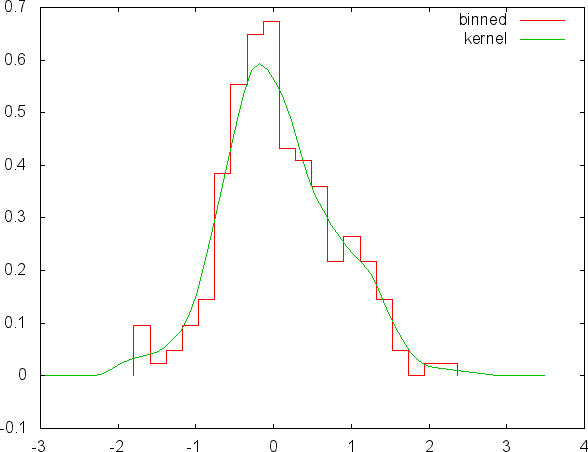
\includegraphics[width=.9\linewidth]{./example1.png}
\caption{\label{Figure-1}Empirical density estimates: binned distribution and kernel estimate}
\end{figure}

Let us see some examples. Figure 1 reports empirical estimates of the
density of $200$ realizations of a exponential power random variable,
obtained using both a binned distribution and a kernel estimate. This
picture can be obtained in  terminal with the following list of commands:
\begin{verbatim}
gbrand -c 1 -r 200 gaussian 1 > data.txt

gbker < data.txt >kernel.txt

gbhisto -n 20 -M 2 <data.txt > histogram.txt 

gbplot -T 'png enhan crop' -o example1.png plot 'w histeps title "binned",\
"kernel.txt" w l title "kernel" ' < histogram.txt

rm data.dat kernel.txt histogram.txt
\end{verbatim}
In the first line, a sample of 200 observations is independently drawn
form a Gaussian distribution with unit variance and saved in the file
\verb~data.txt~. The second line builds a kernel estimate of the density
and the third an histograms. Results are saved in \verb~kernel.txt~ and
\verb~histogram.txt~, respectively. The command in the fourth line, which
continues on the fifth, generates the plot and save the result in
\verb~example1.png~ and the last line remove all the intermediary files.


\begin{figure}[htb]
\centering
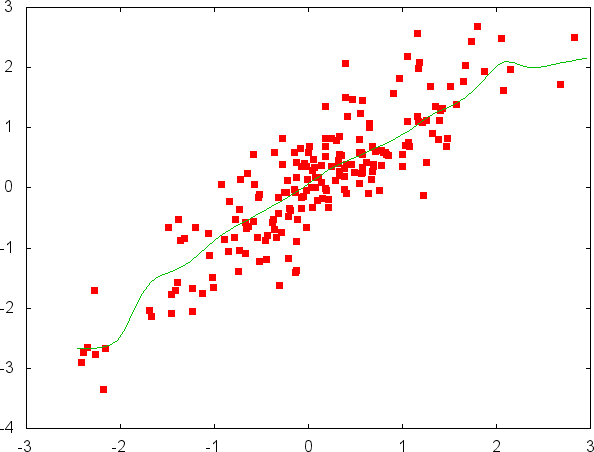
\includegraphics[width=.9\linewidth]{./example2.png}
\caption{\label{Figure-2}Scatter plot and non-linear regression}
\end{figure}
The second example, Figure 2, is a scatter plot of couples of points
together with a non-linear kernel regression. 
\begin{verbatim}
gbrand -c 2 -r 200 gaussian 1 | gbfun 'x1' 'x1+.5*x2' > data.txt

gbkreg < data.txt > kernel_reg.txt

gbplot -T 'png enhan crop' -o example2.png plot 'w p pt 5,\
"kernel_reg.txt" w l ' < data.txt

rm kernel_reg.txt data.txt
\end{verbatim}
The data generated in the first line and saved in \verb~data.txt~ are
independent couples of correlated random variables. A kernel
regression is performed in the second line. The third (and fourth)
lines produce the plot.


What these commands do is to generate random samples, somehow
manipulate them, perform some model estimation and finally plot the
result. All this in one line of code. 

Both pictures are generated using \texttt{gbplot}, which is an interface to
the \href{http://www.gnuplot.info/}{gnuplot} graphic program. To reproduce these pictures the latter
must be installed in your system. Grasping all the details of the
lines above is probably complicated. The baseline message, whoever,
should be clear: even complicated analysis can be split in a sequence
of very simple steps.

The programs in \verb~gbutils~ are completely written in C. Some of them
can make use of external libraries (see below).

These programs have been tested (and repeatedly used for many years)
on different Linux distributions and should compile and run, in
principle, on any Unix platform. Other operating systems, most notably
Windows, have been scarcely tested.

These programs have been originally written for personal use. Even if
today they are used by several persons, please consider that I
maintain and develop them in my spare time. They are distributed under
the \href{COPYING}{GPL license} in the hope they could be of help to other people, but
without any implied warranty.

Please report bugs to \url{mailto:gbutils@googlegroups.com}

\subsection{Requirements}
\label{sec-1-1}

To be installed from source, the package requires a C compiler and the
standard C library. Unix-like environment in which GNU auto-tools can
work is required for automatic installation.

Many programs in gbutils do not require ANY external library apart the
standard ones. There are however exceptions. Several programs use the
GNU Scientific Library (GSL) (version >= 1.6) and other the GNU
matheval library (version >=1.0.1).

See the "Programs summary table" for the list of dependencies of the
different utilities.

At install time, if a library is not found, the programs requiring it
are omitted from the list of programs to be installed.

If the zlib library is found on the system, all the utilities are
compiled with the capability of reading gz-compressed input.

For more information about GSL, including installation procedures on
various platforms, check \href{http://www.gnu.org/software/gsl/}{here}.  GNU matheval library is hosted \href{http://savannah.gnu.org}{here}
and zlib home page is \href{http://www.gzip.org/zlib/}{here}.

Notice that, in principle, using programs linked with different
libraries can produce slightly different outputs.
\subsection{Installation instructions}
\label{sec-1-2}

On \texttt{Linux}, the \texttt{gbutils} package can be either installed using a .deb
package or from source. The first method is recommended. You can
download the binaries executable for your system from the \href{https://packages.debian.org/unstable/main/gbutils}{Debian} or
the \href{http://packages.ubuntu.com/wily/gbutils}{Ubuntu} repositories. Alternatively, the latest source code is
available from the \href{ftp://cafed.sssup.it/packages/}{cafed} repository. Check the \verb~README~ file in the
distributed package for instruction about the installation from
source.

In \texttt{Windows}, the \texttt{gbutils} package is installed in the \texttt{Cygwin}
environment. Follow the instructions in the \href{http://cafim.sssup.it/~giulio/software/gbutils/cygwin_install.html}{cygwin installation} page.
\section{Documentation}
\label{sec-2}

For a brief survey of the package features see the \href{http://cafim.sssup.it/~giulio/software/gbutils/overview.html}{overview}. The
\texttt{gbget} utility is the Swiss knife of the package, the main tool to
perform data manipulation. Its special role commands a specific \href{http://cafim.sssup.it/~giulio/software/gbutils/gbget.html}{gbget
tutorial}.

A brief summary of options and modes of operation can be obtained from
all the programs using the command line option \verb~-h~ or \verb~--help~. All
the programs are accompanied by automatically generated manual pages
which can be isnpected with the \texttt{man} Unix utility.
\section{Contributors}
\label{sec-3}

\href{http://www1.fee.uva.nl/cendef/whoiswho/showHP/default.asp?pID=6&selected=pi}{Cees Diks}, \href{http://www.cafed.sssup.it/~federico/}{Federico Tamagni}, \href{http://cafim.sssup.it/~angelo/}{Angelo Secchi} and Davide Pirino provided
helpful suggestions and coding.
% Emacs 24.3.1 (Org mode 8.2.4)
\end{document}